% questions.tex —— 2024 年·新高考Ⅰ卷 · 题目内容片段（无答案）
% 由 tools/generate_projects.py 依来源总账自 2024/2024_数学真题_试题.md 生成，勿手改（改源 MD 后重跑）


\begin{gknotice}
\textbf{结构分水岭}：2024 年起题量由 22 题减为 19 题（多选 4→3、填空 4→3、解答 6→5），单题分值提高、压轴更难。本卷结构与 2025、2026 完全一致，\textbf{是最贴近 2027 高考的对标真题之一}。

\textbf{适用省份}：山东、广东、湖南、湖北、河北、江苏、福建、浙江、河南、江西、安徽
\end{gknotice}

\par\medskip

\gkpart{一、单选题}

\begin{gktip}
本题共 8 小题，每小题 5 分，共 40 分。在每小题给出的四个选项中，只有一项是符合题目要求的。
\end{gktip}

\begin{question}
\gkti{1}已知集合 $A=\left\{x\mid -5<x^{3}<5\right\}$，$B=\{-3,-1,0,2,3\}$，则 $A\cap B=$（　　）

\begin{gkopts}(4)
\task A．$\{-1,0\}$
\task B．$\{2,3\}$
\task C．$\{-3,-1,0\}$
\task D．$\{-1,0,2\}$
\end{gkopts}

\end{question}
\begin{question}
\gkti{2}若 $\dfrac{z}{z-1}=1+\mathrm{i}$，则 $z=$（　　）

\begin{gkopts}(4)
\task A．$-1-\mathrm{i}$
\task B．$-1+\mathrm{i}$
\task C．$1-\mathrm{i}$
\task D．$1+\mathrm{i}$
\end{gkopts}

\end{question}
\begin{question}
\gkti{3}已知向量 $\boldsymbol a=(0,1)$，$\boldsymbol b=(2,x)$，若 $\boldsymbol b\perp(\boldsymbol b-4\boldsymbol a)$，则 $x=$（　　）

\begin{gkopts}(4)
\task A．$-2$
\task B．$-1$
\task C．$1$
\task D．$2$
\end{gkopts}

\end{question}
\begin{question}
\gkti{4}已知 $\cos(\alpha+\beta)=m$，$\tan\alpha\tan\beta=2$，则 $\cos(\alpha-\beta)=$（　　）

\begin{gkopts}(4)
\task A．$-3m$
\task B．$-\dfrac m3$
\task C．$\dfrac m3$
\task D．$3m$
\end{gkopts}

\end{question}
\begin{question}
\gkti{5}已知圆柱和圆锥的底面半径相等，侧面积相等，且它们的高均为 $\sqrt3$，则圆锥的体积为（　　）

\begin{gkopts}(4)
\task A．$2\sqrt3\pi$
\task B．$3\sqrt3\pi$
\task C．$6\sqrt3\pi$
\task D．$9\sqrt3\pi$
\end{gkopts}

\end{question}
\begin{question}
\gkti{6}已知函数 $f(x)=\begin{cases}-x^{2}-2ax-a,&x<0\\ \mathrm{e}^{x}+\ln(x+1),&x\ge0\end{cases}$ 在 $\mathbf R$ 上单调递增，则 $a$ 的取值范围是（　　）

\begin{gkopts}(4)
\task A．$(-\infty,0]$
\task B．$[-1,0]$
\task C．$[-1,1]$
\task D．$[0,+\infty)$
\end{gkopts}

\end{question}
\begin{question}
\gkti{7}当 $x\in[0,2\pi]$ 时，曲线 $y=\sin x$ 与 $y=2\sin\left(3x-\dfrac{\pi}{6}\right)$ 的交点个数为（　　）

\begin{gkopts}(4)
\task A．$3$
\task B．$4$
\task C．$6$
\task D．$8$
\end{gkopts}

\end{question}
\begin{question}
\gkti{8}已知函数 $f(x)$ 的定义域为 $\mathbf R$，$f(x)>f(x-1)+f(x-2)$，且当 $x<3$ 时 $f(x)=x$，则下列结论中一定正确的是（　　）

\begin{gkopts}(4)
\task A．$f(10)>100$
\task B．$f(20)>1000$
\task C．$f(10)<1000$
\task D．$f(20)<10000$
\end{gkopts}

\par\medskip

\end{question}
\gkpart{二、多选题}

\begin{gktip}
本题共 3 小题，每小题 6 分，共 18 分。全部选对得 6 分，部分选对得部分分，有选错得 0 分。
\end{gktip}

\begin{question}
\gkti{9}随着"一带一路"国际合作的深入，某茶叶种植区多措并举推动茶叶出口。为了解推动出口后的亩收入（单位：万元）情况，从该种植区抽取样本，得到推动出口后亩收入的样本均值 $\bar x=2.1$，样本方差 $s^{2}=0.01$。已知该种植区以往的亩收入 $X$ 服从正态分布 $N\left(1.8,\ 0.1^{2}\right)$，假设推动出口后的亩收入 $Y$ 服从正态分布 $N\left(\bar x,\ s^{2}\right)$，则（若随机变量 $Z$ 服从正态分布 $N\left(\mu,\sigma^{2}\right)$，则 $P(Z<\mu+\sigma)\approx0.8413$）（　　）

\begin{gkopts}(4)
\task A．$P(X>2)>0.2$
\task B．$P(X>2)<0.5$
\task C．$P(Y>2)>0.5$
\task D．$P(Y>2)<0.8$
\end{gkopts}

\end{question}
\begin{question}
\gkti{10}设函数 $f(x)=(x-1)^{2}(x-4)$，则（　　）

\begin{gkopts}(2)
\task A．$x=3$ 是 $f(x)$ 的极小值点
\task B．当 $0<x<1$ 时，$f(x)<f\left(x^{2}\right)$
\task C．当 $1<x<2$ 时，$-4<f(2x-1)<0$
\task D．当 $-1<x<0$ 时，$f(2-x)>f(x)$
\end{gkopts}

\end{question}
\begin{question}
\gkti{11}设计一条美丽的丝带，其造型可以看作图中曲线 $C$ 的一部分。已知 $C$ 过坐标原点 $O$，且 $C$ 上的点满足：横坐标大于 $-2$；到点 $F(2,0)$ 的距离与到定直线 $x=a\ (a<0)$ 的距离之积为 $4$，则（　　）

\begin{center}% 2024 新高考Ⅰ卷 11："丝带"曲线 C：((x-2)^2+y^2)·(x+2)^2=16（过原点，a=-2）
% 由 y=±sqrt(16/(x+2)^2-(x-2)^2) 精确绘制；x→-2 时 y→∞，绘图窗口截断
\begin{tikzpicture}
\begin{axis}[width=7.6cm, height=6.6cm, font=\small,
  axis lines=middle, xlabel={$x$}, ylabel={$y$},
  xmin=-3.1, xmax=4.1, ymin=-3.1, ymax=3.1,
  xtick=\empty, ytick=\empty,
  every axis x label/.style={at={(current axis.right of origin)}, anchor=west},
  every axis y label/.style={at={(current axis.above origin)}, anchor=south}]
  \addplot[domain=-1.75:2.8284, samples=300, thick]
    { sqrt(max(0, 16/((x+2)^2) - (x-2)^2)) };
  \addplot[domain=-1.75:2.8284, samples=300, thick]
    {-sqrt(max(0, 16/((x+2)^2) - (x-2)^2)) };
  \node[below left] at (axis cs:0,0) {$O$};
  \fill (axis cs:2,0) circle (1.2pt) node[below] {$F$};
  \node at (axis cs:-1.3,2.5) {$C$};
\end{axis}
\end{tikzpicture}
\end{center}

\begin{gkopts}(1)
\task A．$a=-2$
\task B．点 $\left(2\sqrt2,0\right)$ 在 $C$ 上
\task C．$C$ 在第一象限的点的纵坐标的最大值为 $1$
\task D．当点 $\left(x_0,y_0\right)$ 在 $C$ 上时，$y_0\le\dfrac{4}{x_0+2}$
\end{gkopts}

\par\medskip

\end{question}
\gkpart{三、填空题}

\begin{gktip}
本题共 3 小题，每小题 5 分，共 15 分。
\end{gktip}

\begin{question}
\gkti{12}设双曲线 $C:\dfrac{x^{2}}{a^{2}}-\dfrac{y^{2}}{b^{2}}=1\ (a>0,\ b>0)$ 的左、右焦点分别为 $F_1$，$F_2$，过 $F_2$ 作平行于 $y$ 轴的直线交 $C$ 于 $A$，$B$ 两点。若 $|F_1A|=13$，$|AB|=10$，则 $C$ 的离心率为 \gkblank{}．

\end{question}
\begin{question}
\gkti{13}若曲线 $y=\mathrm{e}^{x}+x$ 在点 $(0,1)$ 处的切线也是曲线 $y=\ln(x+1)+a$ 的切线，则 $a=$ \gkblank{}．

\end{question}
\begin{question}
\gkti{14}甲、乙两人各有四张卡片，每张卡片上标有一个数字，甲的卡片上分别标有数字 $1,3,5,7$，乙的卡片上分别标有数字 $2,4,6,8$。两人进行四轮比赛。在每轮比赛中，两人各自从自己持有的卡片中随机选一张，并比较所选卡片上数字的大小，数字大的人得 $1$ 分，数字小的人得 $0$ 分，然后各自弃置此轮所选的卡片（弃置的卡片在此后的轮次中不能使用）。则四轮比赛后，甲的总得分不小于 $2$ 的概率为 \gkblank{}．

\par\medskip

\end{question}
\gkpart{四、解答题}

\begin{gktip}
本题共 5 小题，共 77 分。解答应写出文字说明、证明过程或演算步骤。
\end{gktip}

\begin{question}
\gkti{15}\textbf{（13 分）} 记 $\triangle ABC$ 的内角 $A$，$B$，$C$ 的对边分别为 $a$，$b$，$c$。已知 $\sin C=\sqrt2\cos B$，$a^{2}+b^{2}-c^{2}=\sqrt2\,ab$。

  (1) 求 $B$；

  (2) 若 $\triangle ABC$ 的面积为 $3+\sqrt3$，求 $c$。

\end{question}
\begin{question}
\gkti{16}\textbf{（15 分）} 已知 $A(0,3)$ 和 $P\left(3,\dfrac32\right)$ 为椭圆 $C:\dfrac{x^{2}}{a^{2}}+\dfrac{y^{2}}{b^{2}}=1\ (a>b>0)$ 上两点。

  (1) 求 $C$ 的离心率；

  (2) 若过 $P$ 的直线 $l$ 交 $C$ 于另一点 $B$，且 $\triangle ABP$ 的面积为 $9$，求 $l$ 的方程。

\end{question}
\begin{question}
\gkti{17}\textbf{（15 分）} 如图，四棱锥 $P\text{-}ABCD$ 中，$PA\perp$ 底面 $ABCD$，$PA=AC=2$，$BC=1$，$AB=\sqrt3$。

\begin{center}% 2024 新高考Ⅰ卷 17：四棱锥 P-ABCD（PA⊥底面 ABCD）
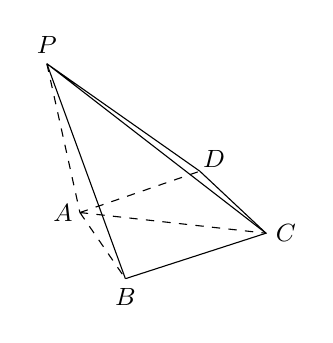
\begin{tikzpicture}[scale=1.05, font=\small]
  \coordinate (P) at (0.75,2.6);
  \coordinate (A) at (1.15,0.8);
  \coordinate (B) at (1.7,0);
  \coordinate (C) at (3.4,0.55);
  \coordinate (D) at (2.6,1.3);
  \draw (P) -- (B)  (P) -- (C)  (P) -- (D);
  \draw (B) -- (C) -- (D);
  \draw[dashed] (P) -- (A);
  \draw[dashed] (A) -- (B)  (A) -- (D)  (A) -- (C);
  \node[above] at (P) {$P$};
  \node[left, inner sep=2.5pt] at (A) {$A$};
  \node[below] at (B) {$B$};
  \node[right] at (C) {$C$};
  \node[above right, inner sep=1pt] at (D) {$D$};
\end{tikzpicture}
\end{center}

  (1) 若 $AD\perp PB$，证明：$AD\parallel$ 平面 $PBC$；

  (2) 若 $AD\perp DC$，且二面角 $A\text{-}CP\text{-}D$ 的正弦值为 $\dfrac{\sqrt{42}}{7}$，求 $AD$。

\end{question}
\begin{question}
\gkti{18}\textbf{（17 分）} 已知函数 $f(x)=\ln\dfrac{x}{2-x}+ax+b(x-1)^{3}$。

  (1) 若 $b=0$，且 $f'(x)\ge0$，求 $a$ 的最小值；

  (2) 证明：曲线 $y=f(x)$ 是中心对称图形；

  (3) 若 $f(x)>-2$ 当且仅当 $1<x<2$，求 $b$ 的取值范围。

\end{question}
\begin{question}
\gkti{19}\textbf{（17 分）} 设 $m$ 为正整数，数列 $a_1,a_2,\cdots,a_{4m+2}$ 是公差不为 $0$ 的等差数列。若从中删去两项 $a_i$ 和 $a_j\ (i<j)$ 后剩余的 $4m$ 项可被平均分为 $m$ 组，且每组的 $4$ 个数都能构成等差数列，则称数列 $a_1,a_2,\cdots,a_{4m+2}$ 是 $(i,j)$-\textbf{可分数列}。

  (1) 写出所有的 $(i,j)$，$1\le i<j\le6$，使得数列 $a_1,a_2,\cdots,a_6$ 是 $(i,j)$-可分数列；

  (2) 当 $m\ge3$ 时，证明：数列 $a_1,a_2,\cdots,a_{4m+2}$ 是 $(2,13)$-可分数列；

  (3) 从 $1,2,\cdots,4m+2$ 中一次任取两个数 $i$ 和 $j\ (i<j)$，记数列 $a_1,a_2,\cdots,a_{4m+2}$ 是 $(i,j)$-可分数列的概率为 $P_m$，证明：$P_m>\dfrac18$。

\par\medskip


\end{question}